\documentclass[12pt,a4paper]{article}

\usepackage[a4paper, top = 2cm, bottom = 2cm, left = 1.5cm, right = 1.5cm]{geometry}
\usepackage[dvipsnames]{xcolor} % Colors

\usepackage{standalone}

\usepackage{setspace}
\usepackage{graphicx}
\usepackage{amsfonts}
\usepackage{amsmath}
\usepackage{tikz}
\usepackage{pdfpages}
\usepackage{epigraph}
\usepackage{csquotes}
\usepackage{natbib}
\usepackage{accents}
\usepackage{pdfpages}

% Bibliography
\usepackage{xcolor}
\usepackage{hyperref}
\hypersetup{
colorlinks=true,
citecolor=MidnightBlue,
linkcolor=MidnightBlue,
pdfpagemode=FullScreen}

\usepackage{listings}
\lstset{frame=tb,
  language=Matlab,
  aboveskip=3mm,
  belowskip=3mm,
  showstringspaces=false,
  columns=flexible,
  basicstyle={\small\ttfamily},
  numbers=none,
  numberstyle=\tiny\color{gray},
  keywordstyle=\color{Red},
  commentstyle=\color{MidnightBlue},
  stringstyle=\color{Red},
  breaklines=true,
  breakatwhitespace=true,
  tabsize=3
}

\usepackage{natbib}
\usepackage[noabbrev]{cleveref}
\setcitestyle{authoryear,open={(},close={)}}
\bibliographystyle{plainnat}

\usepackage{subfiles}

\usepackage{url}
\urlstyle{same} % omit this command if you want monospaced-font look
\newcommand\purl[1]{\protect\url{#1}} % "protected url"

\setlength\parindent{0pt}
\spacing{1.2}

\begin{document}

\begin{center}
       \vspace*{4cm}
       \huge\textbf{Project 5} \\
       \vspace{0.4cm}
       \large \textbf{Public Finance in Macroeconomics} \\
       \vspace{0.5cm}
        \large Handed in by the \textcolor{orange}{\textbf{Heterogeneous Geeks}} \\
        \vspace{0.3cm}
        a.k.a. Vivien Voigt, Thong Nguyen, 
\includegraphics[scale=0.06]{geek.png}\\Davide Difino \& Celina Proffen \\
       \vspace{1.5cm}
       \vfill



        Project in the context of Prof. Ludwig's course: \\
        \textbf{Public Finance in Macroeconomics: Heterogenous Agent Models}\\
        at the Graduate School of Economics, Finance, and Management
       \vspace{0.8cm}
   \end{center}

\newpage

%-----------------------------------------------------

\section{Solution}

\subsection{Explain all sections of the code}

The main function presented in {\fontfamily{ccr}\selectfont towards\_olg} are:

\begin{lstlisting}[frame=single]
% -------------------------------------------------------------------------------%
% use all functions below to print graphs
function towards_olg
% -------------------------------------------------------------------------------%

% -------------------------------------------------------------------------------%
% define the values of parameters
function func_calibr(opt_det,opt_nosr,opt_ny)
% ------------------------------------------------------------------------------- %

% ------------------------------------------------------------------------------- %
% solution of the household problem
%    prints:
%       - state variable matrix (gridx)
%       - saving grid (gridsav)
%       - optimal consumption function (cfun)
%       - optimal value function (vfun)
function [gridx,gridsav,gridass,cfun,vfun] = func_hh
% ------------------------------------------------------------------------------- %

% ------------------------------------------------------------------------------- %
% aggregation and cross-sectional measure
%   prints:
%       - distribution of assets conditional by age and shock (Phi)
%       - distribution of assets (PhiAss)
function [Phi,PhiAss,ass]=func_aggr(gridx,gridsav,cfun,gridass)
% ------------------------------------------------------------------------------- %

% ------------------------------------------------------------------------------- %
% compute average life-cycle profiles
function [labinclife,inclife,asslife,conslife,vallife] = lcprofile(Phi,gridass,cfun,vfun)
% ------------------------------------------------------------------------------- %

% ------------------------------------------------------------------------------- %
% utility function
function u = U(c)
% ------------------------------------------------------------------------------- %
\end{lstlisting}
\pagebreak
\begin{lstlisting}[frame=single]
% ------------------------------------------------------------------------------- %
% marginal utility function
function muc=MUc(c)
% ------------------------------------------------------------------------------- %

% ------------------------------------------------------------------------------- %
% construction of the Markov chain process
%   prints:
%       - transition matrix first eigenvector (pini)
%       - shocks values (gridy)
%       - transition matrix (pi)
function [pini,pi,gridy]=mchain(rhoeta,epsil)
% ------------------------------------------------------------------------------- %

% ------------------------------------------------------------------------------- %
% this function computes the inverted of the utility function
% it is required in func_hh to retrive optimal consumption from the value function
function invut=invut(marg)
% ------------------------------------------------------------------------------- %

% ------------------------------------------------------------------------------- %
% create curved grid using curvature parameter c
function grd = makegrid(x1,x2,n,c)
% ------------------------------------------------------------------------------- %
\end{lstlisting}

For a more detailed description, please refer to {\fontfamily{ccr}\selectfont toward\_olg\_commented}.

\subsection{}

The solution procedure in {\fontfamily{ccr}\selectfont func\_hh} uses the "endogenous gridpoints approach" for solving dynamic stochastic optimization problems, as introduced by \citeauthor{carroll2002lecture} (\citeyear{carroll2002lecture}, \citeyear{carroll2006method}). Instead of creating using an "exogenous" - in that it is given by the coder - grid for the state variable cash-on-hand ($x$), the "endogenous" approach exploit the definion

$$ s = x - c $$

- that is, (end of period) savings are equal to cash-on-hand minus consumption - to compute a new cash-on-hand grid in each period of iteration (over time and possible shock realization), given a fixed (and "exogenous") grid for $s$. Furthermore, substituting $s$ into the Euler equation allows to solve easily for consumption for each point of the saving grid. That is, for each iteration, a pair $s$ and $c(s)$ is defined. The endogenous cash-on-hand grid is then $x(s) = s + c(s)$, and represent the level of cash-on-hand that are rquired for each level of end-of-period savings (and optimal consumption given saving target). Then the value function in current period is updated for each value of the new endogenous cash-on-hand grid (given age and shock, still) by interpolation.

The exogenous grid approach, on the other hand, does both the derivation of the conditional policy function and the updating of the value function at the end of the iteration on the endogenous grid.

The advantages of the exogenous grid method are twofold: first of all, it does not require a nonlinear rootfinding since the Euler equation is solved for $c$ given $s$, instead of $x$, thus removing consumption from the RHS. Second, updating the value function over the endogenous grid for $x$ is more efficient in that the value function ($V'$) is interpolated only for values of $x'$ that have been used to compute $c'$ in the first istance, while the exogenous approch loops over \textit{all} possible $x'$.

\subsection{}

Please refer to {\fontfamily{ccr}\selectfont toward\_olg\_exogenous}

\subsection{}

Please refer to {\fontfamily{ccr}\selectfont toward\_olg\_not\_first\_order}

\subsection{}

\textbf{What is the role of the objects TT and Phi?}

Firstly, for this exercise, we need to understand even more clearly how pi, pini and gridy look like. They are explained in the mchain function.

\begin{lstlisting}[frame=single]
[pini,pi,gridy]=mchain(rhoeta,epsil);

% pi are Transition Probabilities. You always have 1- rhoeta probability of remaining in you current state.. although i find it weird that the off-diagonal elements are also one
pi=rhoeta*ones(2,2);
pi(1,2)=1.0-rhoeta;
pi(2,1)=1.0-rhoeta;

% gridy are rescaled income shocks such that mean is one
gridy=zeros(2,1);
gridy(1)=exp(1.0-epsil);
gridy(2)=exp(1.0+epsil);
gridy=2.0*gridy/(sum(gridy));

% pini is Initial Distribution
pini=0.5*ones(2,1);
\end{lstlisting}

Okay, so now that this is clear, let's try to explain the role of TT and Phi! Both these objects are defined and used in lines 402-434 in the code, which is why  inserted the corresponding section below:

\begin{lstlisting}[frame=single]
    function [Phi,PhiAss,ass]=func_aggr(gridx,gridsav,cfun,gridass)

    global r nj nx ny pi gridy netw pens sr epsi pini frac totpop

    disp('aggregation and cross-sectional measure');

    % Compute Cross sectional distributions and aggregate variables
    Phi = zeros(nj,ny,nx);          % distribution of assets conditional by age and shock
    PhiAss = zeros(nx,1);             % distribution of assets

    % Distribution of newborns over cash at hand
    for yc=1:ny

        % income (wages and pensions) in current period/age:
        inc=epsi(1)*netw*gridy(yc)+(1-epsi(1))*pens;

        % initial cash-on-hand:
        cahini=inc;

        [vals,inds]=basefun(gridx(1,yc,:),cahini,nx);
        Phi(1,yc,inds(1))=vals(1)*pini(yc)*frac(1);
        Phi(1,yc,inds(2))=vals(2)*pini(yc)*frac(1);
    end;

    for jc=2:nj
        TT = zeros(ny,nx,ny,nx);    % transfer function

        for xc=1:nx
            for yc=1:ny
                for ycc=1:ny

                    % income (wages and pensions) in current period/age:
                    inc=epsi(jc)*netw*gridy(ycc)+(1-epsi(jc))*pens;

                    % cash on hand: x=a*(1+r)+y = s(-1)*(1+r)+y;
                    cah=inc+(1.0+r)*gridsav(xc);

                    [vals,inds]=basefun(gridx(jc,ycc,:),cah,nx);

                    TT(ycc,inds(1),yc,xc)=vals(1)*pi(yc,ycc);
                    TT(ycc,inds(2),yc,xc)=vals(2)*pi(yc,ycc);
                end;
            end;
        end;

        for xc=1:nx
            for yc=1:ny
                for xcc=1:nx
                    for ycc=1:ny
                        % transfer distribution:
                        Phi(jc,ycc,xcc)=Phi(jc,ycc,xcc)+Phi(jc-1,yc,xc)*TT(ycc,xcc,yc,xc)*sr(jc-1);
                    end;
                end;
            end;
        end;

    end;    % end for jc


\end{lstlisting}

First notice that Phi has three dimensions: It accounts for age, the current state of income shocks and the level of cah that individuals hold. In the first period of life we know how assets are distributed, as we assume that initial assets are generated with the same process ass income. Basically, everyone starts off with some assets that amount to the income realization people had in the past period, i.e. $t=0-1$. The initial distribution at age 1 is again state dependent; i.e. we could start of with any of these two states; which explains that there could be differences in the aggregate asset distribution over the entire life cycle due to the (randomly selected) state you start off in. \\

Then, next TT is the transfer function that is defined for most periods in time, or - more precisely - for the nj-1 times that the people transition into the next age group. TT is build up in 4 layers. To explain them,  will denote them as follows $TT(ny,nx,ny,nx)=TT(ycc, xc\_new,yc,xc\_old))$.\\

We need to define TT for all age groups, which is done by simply creating a new TT for all current ages. Given each age, one might be holding different levels of cah, which is what we do though the xc\_old index. In the last period, each person's income was dependent on a shock yc, which needs to be accounted for as the past shock will determine the probability of one's next shock (remember that these estimates are stored in pi(yc,ycc) which gives the transition probability from state yc to ycc). Given a past shock, we can compute the income for any of the new shocks ycc that might hit us.  That income times the interest rate plus the savings associated with the given level of cah xc\_old will determine the cah in the next period. In the transition matrix we will now store the expected probability of transitioning into state xc\_new in the coming period. \\

Note: The last part is done by relying on the basefun and lookup functions. What they basically do here, is to estimate the cah level you will get in next period. As this will usually not be a precise gridpoint of gridx, we assign a positive probability to the gridpoint just above and just below the new cah estimate. :) \\

In a final step for each age you fill out the new Phi distribution for all past states of shock realizations and cah holdings. The proability of dying early is also accounted for.\\

\textbf{Compare this with the corresponding definitions in the lecture notes:} \\
This is actually really hard to do, because our transition matrix in the Markov process is very simple. We can basically apply the same transition process at all ages, in the sense that multiplying it with the current shock distribution, will give us a matrix with the new distribution of income shock realizations. \\

In terms of Phi, we do not really have an assumption about the initial state of assets in the lecture notes. Rather, it is suggested that we may run simulations and average over them.

\textbf{Code modification}
The project instructions ask us to implement a more efficient way for looping over all the different states. we did so, as you can see in the attached matlab file named "Solution\_1.5"

The time elapsed now was:

\begin{lstlisting}
    time elapsed: 9.3518
\end{lstlisting}

vs. the time before:

\begin{lstlisting}
    time elapsed: 11.5845
\end{lstlisting}

(It is to note however, that the milliseconds vary across different times. The above times are more or less a medium measure of how long each script takes. )

\subsection{}
\textbf{Comparison of Models}

In the attached PDF (Comparison model outcomes) we plotted all required scenarios in a way that (hopefully) allows an easier comparison\footnote{The asset distribution at different ages was cut down to just display it at age 80 out of space constraints.}. We have classified the models as follows, whereby the red coloured part identifies the deviations from the standard model:

\begin{itemize}
    \item Standard: opt\_det = false, opt\_nosr = true, tetta=2, r=0.04, rho=0.04
    \item Variation 1: opt\_det = true, opt\_nosr = true, tetta=2, r=0.04, rho=0.04
    \item Variation 2: \textcolor{red}{opt\_det = true, opt\_nosr = false}, tetta=2, r=0.04, rho=0.04
    \item Variation 3: opt\_det = false, \textcolor{red}{opt\_nosr = false}, tetta=2, r=0.04, rho=0.04
    \item Variation 4: opt\_det = false, opt\_nosr = true, \textcolor{red}{tetta=1}, r=0.04, rho=0.04
    \item Variation 5: opt\_det = false, opt\_nosr = true, \textcolor{red}{tetta=5}, r=0.04, rho=0.04
    \item Variation 6: opt\_det = false, opt\_nosr = true, tetta=2, r=0.04, \textcolor{red}{rho=0.4}
    \item Variation 7: opt\_det = false, opt\_nosr = true, tetta=2, \textcolor{red}{r=0.4}, rho=0.04
\end{itemize}

\textbf{The standard model} interest rates and impatience parameter balance each other out, s.t. the left and RHS of the standard Euler equation (w.o. accounting for possible borrowing constraints) simplify to the marginal utility of consumption today having to equal the expected marginal utility of consumption tomorrow. However, there is a precautionary motive turned on given the positive third derivative (presence of prudence) and variability in the income process (it is NOT deterministic but rather modelled by a Markov process). People know for certain when they will die which explains the shape of assets that monotonically approaches zero from above (last part of the asset function over the life cycle is concave). the intuition is, that people do not want to die with left-over assets as they still derive utility from them. \\

\textbf{Variation 1} makes income deterministic, which will turn of the precautionary savings behavior. The distribution of assets is suddenly more dense, i.e. people do not behave so differently in their savings behavior, as they do not experience different income states. They also build up the assets more slowly than they did under the standard specifications. Fianlly, it is to note that there is a massive change in the consumption profile of agents. Looking at the scale that corresponds to the consumption level graph, the changes in absolute consumption are smaller than those in the standard model. The consume their income almost fully until they are about to retire. In the last years of the working life the agents start saving a larger portion (as they become concerned with their retirement time) and during the retirement their consumption remains constant (as it did in the standard model). \\

\textbf{Variation 3} (we will come to Variation 2 next), uses the standard model but now changes besides having stochastic income allows for survival risk (i.e. people never know when they will exactly die). A 100 is however the moment, when one dies with absolute certainty. This survival risk is another source of risk, which can change the consumption pattern. As in the standard model, the asset distribution is rather wide, although a bit lower than in the standard case (people apparently don't want to save as much as before, as they never know whether this means having wasted consumption during the precious time alive ;) Accordingly savings are also a bit lower, and consumption a bit higher than in the standard case. In line with the logic described above, the shape of the consumption function over the life cycle decreases over age (and does not stay constant and high as in the standard model w/o survival risk). \\

\textbf{Variation 2} combines survival risk and a deterministic income process: i.e. we have more risk of dying unpredictably, but save earnings. Again, like in variation 1, the distribution of assets is much more narrow, but this time focuses even more at an early age (when it is still pretty unlikely that one will die).  In comparison to Variation 1, which has no survival risk, we see that the consumption profile is hump-shaped, in line with the idea that one knows that it is ever more unlikely that one will survive and doe snot want to leave too many assets behind without consuming them. In contrast to Variation 3, where income is not deterministic, people only start saving more out of current income as they approach the retirement age. This is in line with the idea, that the labor income during working age (conditional on surviving) will come in in its full/ constant amount for sure.\\

\textbf{Variation 4 and 5}. Looking at Variations 4 and 5, we can make some observations on how tetta, the coefficient of relative risk aversion, changes consumption/ savings behavior in a model of stochastic income but with no survival risk. A higher tetta implies that the RHS of the Euler equation will increase with uncertainty, and that we will want to save more. This is hard to see in the graphs, but there is indeed some differences over the assets accumulated over the life cycle, when one pays close attention to the savings and the assets graph. Also, and perhaps more clearly, the graph on the consumption function over the life cycle reveals that during the retirement age, people with a higher tetta are able to consume more (given their savings).\\

Also note, that 1/tetta= IES, the intertemporal elasticity of substitution. The latter makes people more willing to adapt their consumption intertemporally when they see an important gain (e.g. in interest rates) from doing so. Here, the interest rate and the intertemporal discount factor equal each other out, but we can still see that people with low IES (high tetta) have a somewhat wider asset distribution over the life cycle, while the ones with low tetta (high IES) take advantage of the compounded interest effects, i.e. they focus the distribution of assets more on the younger ages to take more advantage of it later.\\

\textbf{Variation 6 and 7} show how the patterns change when (given a constant tetta) the relationship between interest rates and discount factor change. Call $A = \frac{1+r}{1+\rho}$; a high $A$ should lead to more savings today (i.e. lower consumption, higher marginal utility from consumption today). Variation 6 entails a very low $A$ and indeed has relatively low savings when comparing it to the Standard case. This is exactly opposite in the Variation 7, where savings reach over 20 times the level of variation 6. Instead of the humped shaped consumption that follows for Variation 6, in 7 we observe a steady and almost exponential increase in consumption of the life cycle. From a highly negative value function in the early years, this rises to significantly higher levels than those observed in variation 6 at approx. the age of 30.\\

\textcolor{red}{@someone: Please note that the labor income in Variation 7 looks really odd- maybe we chose parameters that are not consistent at some point. I still think we can use these graphs here, but I would recommend explaining/ understanding why this happened. }

\section*{Problem 2: Calibration}

For this problem, we must keep in mind our results in PS 4. For the sake of completeness, we here reiterate the key findings of that problemset concerning parameters for pre and post government income.

\begin{table}[h]
\begin{tabular}{|l|l|l|}
\hline
\textbf{Variable} & \textbf{Pre government income} & \textbf{Post government income}  \\ \hline
$\rho$                        &   .9652454 (.0546179)  &  .8501573  (.038411)         \\ \hline
$\sigma^2_z$                  &   2.385936 (17.57936)  &  -1729.153 (3620.489)        \\ \hline
$\sigma^2_\nu$                &   .0550472 (.1076207)  &   .2028518 (.0676536)        \\ \hline
$\sigma^2_\epsilon$           &   .3610598  (.084534)  &   .1343607 (.0364851)        \\ \hline
$\sigma^2_{\Tilde{y}}$        &   1.167006             &   .8660633                   \\ \hline
\end{tabular}
\caption{The estimates for all variables but $\sigma^2_{\Tilde{y}}$ stem from estimations in the stata do.file handed in together with this project instructions. The estimate of $\sigma^2_{\Tilde{y}}$ is computed using the formula given in the project instructions and also derived below.}
\end{table}

and from our regression on the cubic in age from project 4, the coefficients are estimated for pre-government (i.e. yhh5, net income) as:

\begin{equation*}
    ln\_yhh5\_hat=8.36501+0.0861011\cdot age-0.0006384 \cdot age^2-0.0000035\cdot age^3+0.4370217\cdot married   
\end{equation*}
\begin{equation*}
    yhh5\_hat=exp(8.36501+0.0861011\cdot age-0.0006384 \cdot age^2-0.0000035\cdot age^3+0.4370217\cdot married)  
\end{equation*}

and for post-government income (yhh6, gross income) as:

\begin{equation*}
    ln\_yhh6\_hat=+8.88529+0.0405944\cdot age+ 0.0002557\cdot age^2-0.0000102\cdot age^3+0.5084652\cdot married  
\end{equation*}
\begin{equation*}
    yhh6\_hat=exp(+8.88529+0.0405944\cdot age+ 0.0002557\cdot age^2-0.0000102\cdot age^3+0.5084652\cdot married  )  
\end{equation*}

\textbf{Exercise 2.1}

From our regression on the cubic in age from project 4, the coefficients are estimated as above. With this we can estimate the age income profile for a given age. (For simplification, we choose $married=0$, we also distinguish between pre-and post-government income.) Since we're only interested in the income from age 20 to 64, we keep the estimates for this age range and set income for all other ages equal 0. After that we can normalize the age profile by dividing income of every age by the average income of the "active earnings" life cycle (i.e. from 20-64 years old). Finally, we replace the age profile in the code with the normalized estimates. Please refer to $\texttt{towards\_olg\_prob\_2.m}$ for the estimates of age profile. \\

The income process we modelled now looks like this for pre-government income: \\
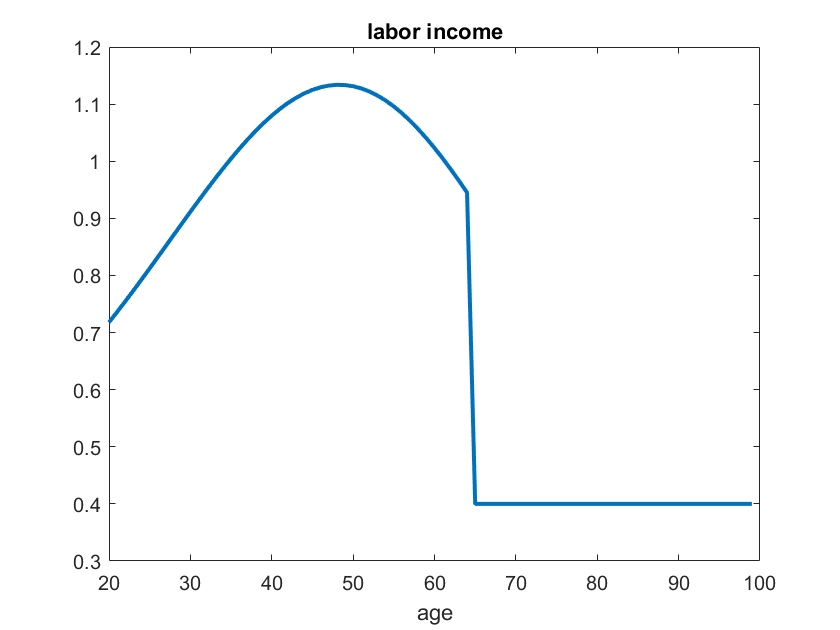
\includegraphics[width=0.6\textwidth]{PS5/Graphs/labor income.png}
\\
If we used the calibration for post-government (i.e. gross income), we achieved the following pattern in labor income:\footnote{As explained below, we used the transition probabilities between labor income shocks as was estimated for yhh5.}\\
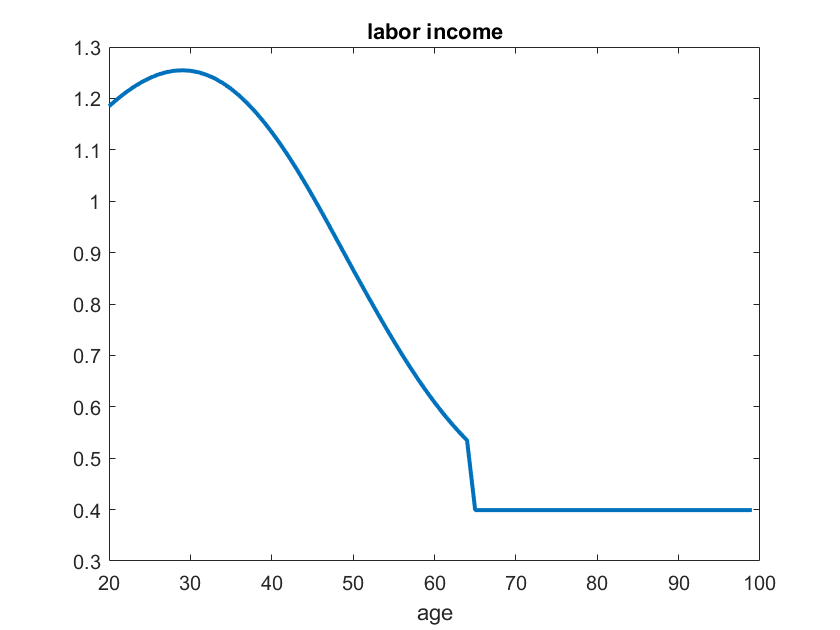
\includegraphics[width=0.6\textwidth]{PS5/Graphs/labor income post gov.png}\\

\textbf{Note:} The project instructions did not want us to calibrate a different income process for pension receivers (it is given as a fixed 0.4 income in the original towards\_old.m code). The resulting graph for labor income looks weird exactly because of this. The government seems to just take working people's money away but does not spend it to feed the elderly more than before. 

\\
\textbf{Exercise 2.2}

\begin{equation}\tag{1a}
     \Tilde{y_t}&=z_t+\epsilon_t 
\end{equation}
\begin{equation}\tag{1b}
    z_t&=\rho z_{t-1} +\nu_t
\end{equation}
Note that (1a) implies:
\begin{equation*}
    z_t=\Tilde{y_t}-\epsilon_t \hspace{5mm} \forall t
\end{equation*}
Therefore from (1b), we have:
\begin{equation*}
    z_{t}=\rho(\Tilde{y}_{t-1}-\epsilon_{t-1})+\nu_t
\end{equation*}
Plugging in (1a) and notice that $\epsilon_t$ and $\nu_t$ are i.i.d:
\begin{equation}\label{one}
    \Tilde{y_t}=\rho(\Tilde{y}_{t-1}-\epsilon_{t-1})+\nu_t+\epsilon_t
\end{equation}
Since the all shocks are orthogonal to each other and the process is weakly stationary, taking the variance yields:
\begin{align*}
    \sigma^2_{\Tilde{y}}&=\rho^2\sigma^2_{\Tilde{y}}+\sigma^2_{\nu}+(1-\rho^2)\sigma^2_{\epsilon}\\
    &=\frac{\sigma^2_\nu}{1-\rho^2} +\sigma^2_\epsilon\\
    &=\sigma^2_z+\sigma^2_\epsilon
\end{align*}
Dividing both sides by $\sigma^2_z$:
\begin{equation*}
    \frac{\sigma^2_{\Tilde{y}}}{\sigma^2_z}=1+\frac{\sigma^2_\epsilon}{\sigma^2_z}
\end{equation*}
Notice that, by i.i.d assumption of shocks from both processes: 
\begin{align*}
    cov(\Tilde{y_t},\Tilde{y}_{t-1})&=cov(\rho z_{t-1} +\nu_t+\epsilon_t,\rho z_{t-2} +\nu_{t-1}+\epsilon_{t-1})=\rho^2cov(z_{t-1},z_{t-2})\\
    cov(z_t,z_{t-1})&=\rho^2cov(z_{t-1},z_{t-2})
\end{align*}
Therefore: \LongRightarrow $cov(\Tilde{y_t},\Tilde{y}_{t-1})=cov(z_{t},z_{t-1})$(*)\\

\textcolor{red}{CP: I don't get how $ cov(z_t,z_{t-1})&=\rho^2cov(z_{t-1},z_{t-2})$ is true? }\\

Furthermore, we have:
\begin{align*}
    \rho_{\Tilde{y}}&=\frac{cov(\Tilde{y_t},\Tilde{y}_{t-1})}{ \sigma^2_{\Tilde{y}}}\\
    \rho&=\frac{cov(z_t,z_{t-1})}{ \sigma^2_z}\\
\end{align*}
Taking the ratio, and from (*), we have:
\begin{equation*}
  \frac{\rho_{\Tilde{y}}}{\rho}=\frac{\sigma^2_z}{\sigma^2_{\Tilde{y}}} =\bigg(1+\frac{\sigma^2_\epsilon}{\sigma^2_z}\bigg)^{-1}
\end{equation*}
Thus: 
\begin{equation*}
\rho_{\Tilde{y}}=\rho\bigg(1+\frac{\sigma^2_\epsilon}{\sigma^2_z}\bigg)^{-1}(Q.E.D)
\end{equation*} 
\textbf{Intuition}: The larger the magnitude of transitory shock relevant to persistent shock, the less variation of $\Tilde{y}$ can be explained by the variation of persistent shock as implied by \eqref{one}, therefore if there were no transitory shock, autocorrelation of $\Tilde{y}$ is equal to that of z, which is $\rho$. Otherwise, $\rho$ should be scaled down by a factor inversely proportional to the ratio of transitory shock and persistent shock, which is $\frac{1}{1+\frac{\sigma^2_\epsilon}{\sigma^2_z}}$\\


\textbf{Calibration with estimates of gross income}\\
\textcolor{red}{@thong: in your calibration I saw different estimates than those we used in project 4.. (I added the table we handed in in project 4 above. Do you see why we have differences there?\\

Also, the project asks us to calibrate everything for two different income processes: yhh5 and yhh6 reliant.. I think we still need to do that for vivien to be able to compute exercise 3 - it should be relatively easy to do by just adding one extra option to the mchain function; i.e. mchain(rho, eta, income_type) and then make the returns of mchain vary according to this option.)}
From estimates in project 4, $\epsilon$ can be calculated as:
\begin{equation*}
    \epsilon=\sigma_{\Tilde{y}}=\sigma_{ln \Tilde{y}}=\sqrt{\frac{\sigma^2_\nu}{1-\rho^2} +\sigma^2_\epsilon}\approx \sqrt{\frac{0.0861262}{1-0.9088825^2} +0.2144817}\approx 0.8424
\end{equation*}
The state vector $[-\epsilon,\epsilon]$ of the logs therefore is: [-0.8424,0.8424]\\
Using the unnumbered equations for $\eta_-$, $\eta_+$ on p.42 of the lecture notes, the the logs can be transformed to levels as: 
\begin{equation*}
    \eta_-=\frac{2exp(1-\sigma_{ln\Tilde{y}})}{exp(1-\sigma_{ln\Tilde{y}})+exp(1+\sigma_{ln\Tilde{y}})}\approx\frac{2exp(1-0.8424)}{exp(1-0.8424)+exp(1+0.8424)}\approx0.3129
    \end{equation*}
    \begin{equation*}
       \eta_+=\frac{2exp(1+\sigma_{ln\Tilde{y}})}{exp(1-\sigma_{ln\Tilde{y}})+exp(1+\sigma_{ln\Tilde{y}})}\approx\frac{2exp(1+0.8424)}{exp(1-0.8424)+exp(1+0.8424)}\approx 1.687 
    \end{equation*}
From previous calibration: $\rho_{\Tilde{y}}=\rho\bigg(1+\frac{\sigma^2_\epsilon}{\sigma^2_z}\bigg)^{-1}\approx0.9088825\bigg(1+\frac{0.2144817}{16.15252}\bigg)^{-1}\approx 0.897 $\\
Using $\kappa=\frac{1+\rho_{\Tilde{y}}}{2}\approx 0.9485$, transition matrix of the Markov process can be calibrated as:\\
\begin{center}
$\Pi$ = \begin{bmatrix}
0.9485 & 0.0515 \\
0.0515 & 0.9485  
\end{bmatrix}
\end{center}\\

Using the estimated values, we can input into the mchain function to implement the model. Please refer to $\texttt{towards\_olg\_prob\_2.m}$ for the implementation. 
    


    
\section*{Problem 3: Analysis}

\section*{Problem 4: Summary of \cite{de2004wealth}}
Since the distribution of wealth is much more concentrated than the distribution of (labour) earnings, De Nardi (2004) estimates a quantitative, general equilibrium, incomplete markets, overlapping-generations model to match this observation from the data. In doing so, the author links parents and children by accidental as well as voluntary bequests - but not by inter vivo transfers - and allows children to inherit some of their parents' productivity. Further, she calibrates the model to match important features of, first, the data of the U.S. and, second, the data of Sweden. Both countries have different wealth distribitions even though their Gini coefficients are relatively similar. This paper's framework makes it possible for intergenerational links to induce saving behaviour that generates a more concentrated distribution of wealth than that of earnings due to allowing two different saving motives: self-insurance against labour earnings shocks and life-span risk, i.e. saving for retirement, which both can be seen as precautionary motives, and the preference to leave bequests to their offspring, which is an altruistic motive.
\\
De Nardi finds that saving for precautionary purposes and saving for retirement are the primary factors for wealth accumulation at the lower tail of the distribution, while saving to leave bequests significantly affects the shape of the upper tail.

\pagebreak

\bibliography{Literature/bibliography.bib}

\pagebreak

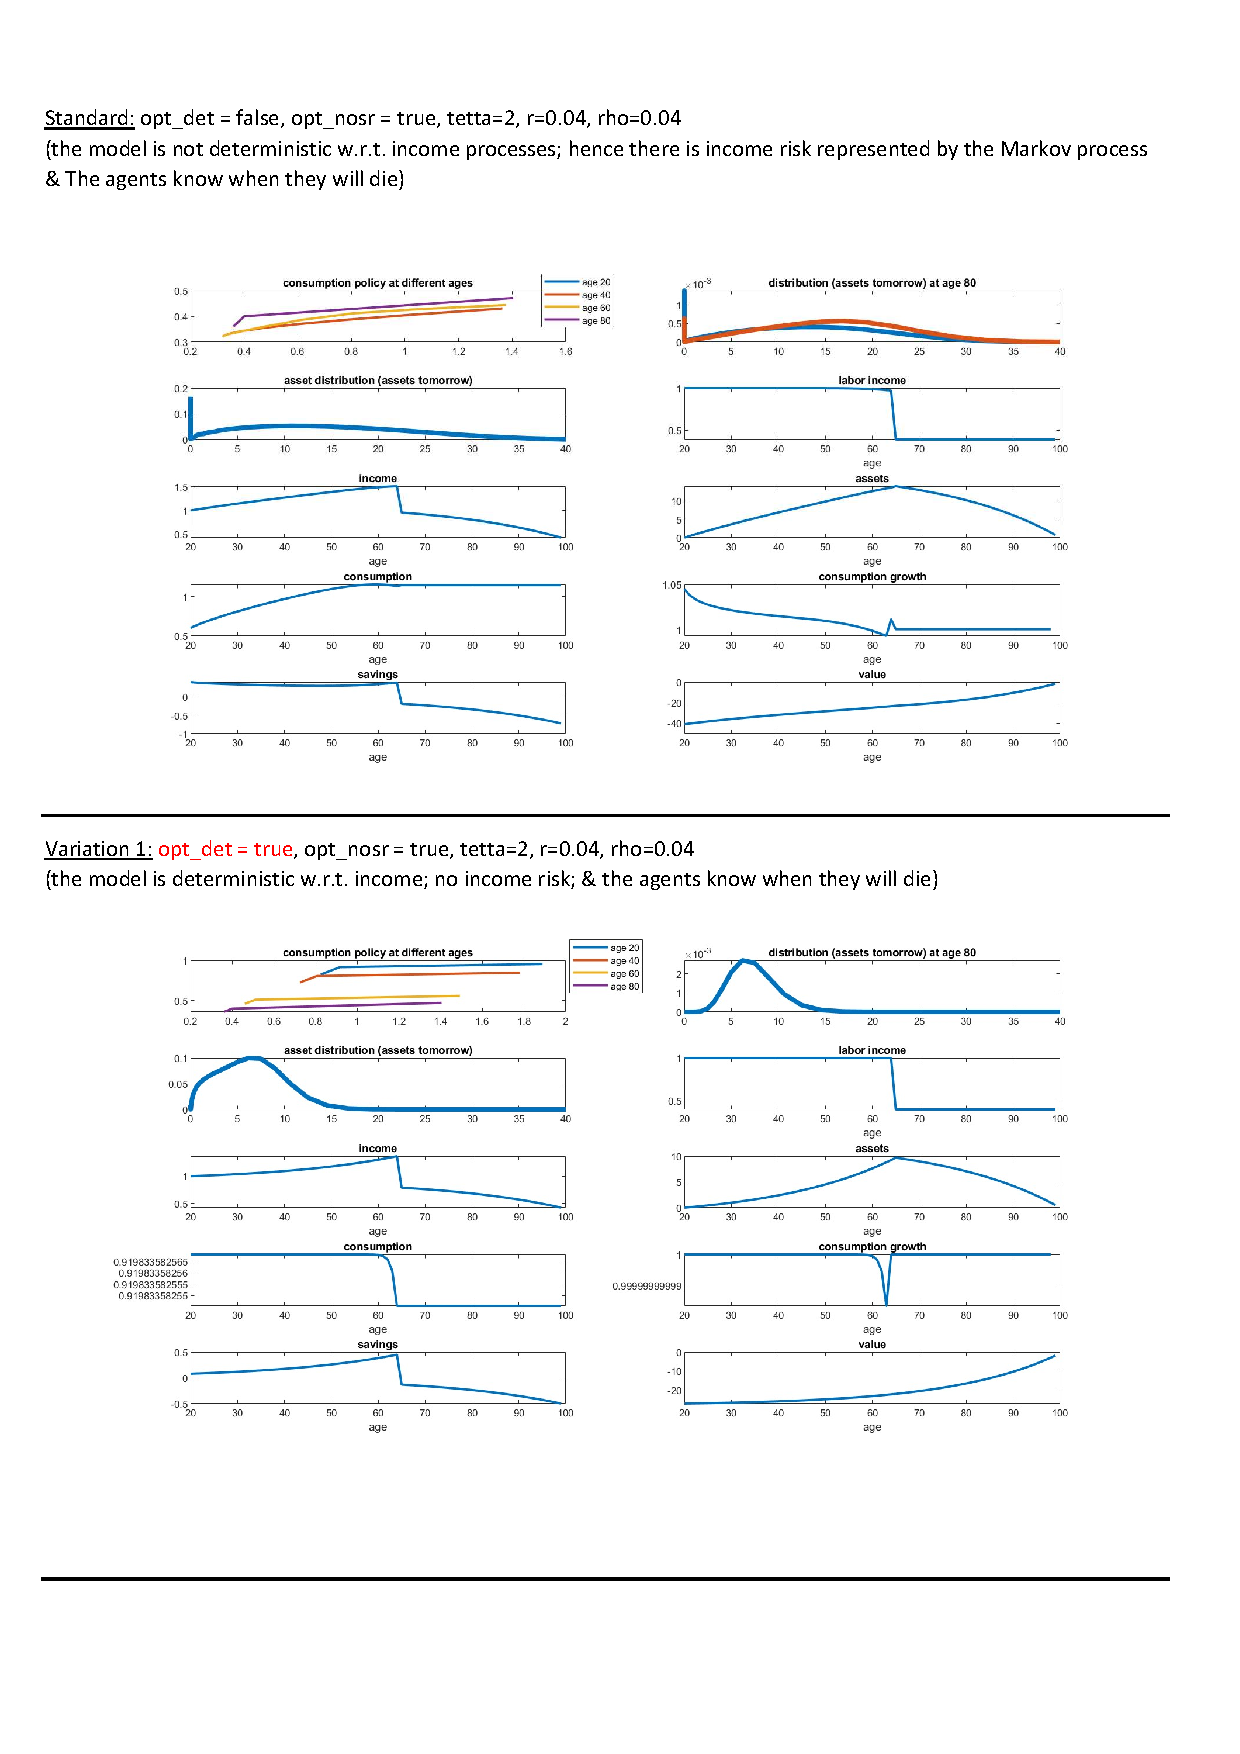
\includepdf[pages=-]{Other documents/Comparison model outcomes.pdf}

\end{document}
